\chapter{Overview of the LHCb upgrade}
\label{ref:lhcb-upgrade-overview}

% General changes
The run 2 of LHC reached its conclusion at the end of 2018,
when it entered the second long shutdown (LS2) period.
Due to luminosity levelling, since 2012,
the LHCb has been collecting data at about 2~fb$^{-1}$ integrated luminosity per
year when the experiment is in a steady state,
with an instantaneous luminosity of about $4 \times 10^{32}$cm$^{-2}$~s$^{-1}$,
far below which the LHC is capable of providing\footnote{
    As a reference, the CMS experiment reached a maximum instantaneous
    luminosity of $1.5 \times 10^{34}$cm$^{-2}$~s$^{-1}$ in 2016.
    % from https://arxiv.org/pdf/2104.01927.pdf
}.
More precise measurements require more data which the current LHCb detector is
unable to provide,
due to the fact that the detector has a limited readout rate of 1~MHz:
even if the instantaneous luminosity is increased,
with current hardware triggers\footnote{
    As discussed in \cref{ref:detector:trigger},
    the hardware triggers require the event to be above a certain $\pt / E_T$
    threshold.
},
to maintain a constant readout rate of 1~MHz,
the thresholds for \pt and $E_T$ have to increase,
which largely cancels the benefit of running at higher luminosity.
As shown in \cref{fig:l0-trigger-eff},
the hadronic trigger yields are saturating even at run 2 luminosity
($4 \times 10^{32}$~cm$^{-2}$~s$^{-1}$).

\begin{figure}[!htb]
    \centering
    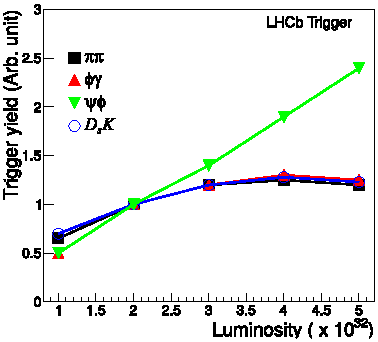
\includegraphics[width=0.5\textwidth]{./figs-lhcb-upgrade-overview/trigger_efficiency.pdf}
    \caption{
        L0 trigger yields normalized to that at
        $2 \times 10^{32}$~cm$^{-2}$s$^{-1}$.
        The hadronic triggers are already saturated at run 2 luminosity.
        Taken from \cite{CERN-LHCC-2011-001}.
    }
    \label{fig:l0-trigger-eff}
\end{figure}

To remove the readout bottleneck,
the detector readout rate is upgraded to 40~MHz,
the LHC bunch crossing rate,
without any hardware trigger.
By exposing all low-level variables to purely software-based high-level
triggers with more exclusive selection criteria,
events can be categorized into exclusive signal decay modes more
efficiently with reasonable write throughputs \cite{Albrecht_2014}.
After the upgrade, the detector will operate at an instantaneous luminosity
of $2 \times 10^{33}$~cm$^{-2}$s$^{-1}$,
a factor of 5 gain compared to that of run 2,
without any hardware trigger,
making LHCb the first (hardware) trigger-less detector.

Aside from the upgrade of the readout system and trigger scheme,
the tracking system is upgraded to provide better resolution and more
radiation tolerance to sustain the increased luminosity.
The subdetectors mainly used in L0 trigger, namely Muon station 1, SPD, and PS,
are removed altogether to reduce material in front of the calorimeters to
improve energy resolution.
The RICH1 detector which is responsible for PID is upgraded to reduce
occupancy\footnote{
    Defined as the fraction of detected photons over the total number of
    channels
    \cite{D_Ambrosio_2017}.
}
thus maintaining good PID efficiency.
The calorimeters (ECAL and HCAL) and the muon system will not undergo
substantial upgrades
\cite{Piucci_2017}.
The changes in the LHCb detector betwen run 1, 2 and run 3 are indicated
in \cref{fig:lhcb-detector-comparison}.

\begin{figure}[!htb]
    \centering
    \begin{subfigure}[t]{0.45\textwidth}
        \centering
        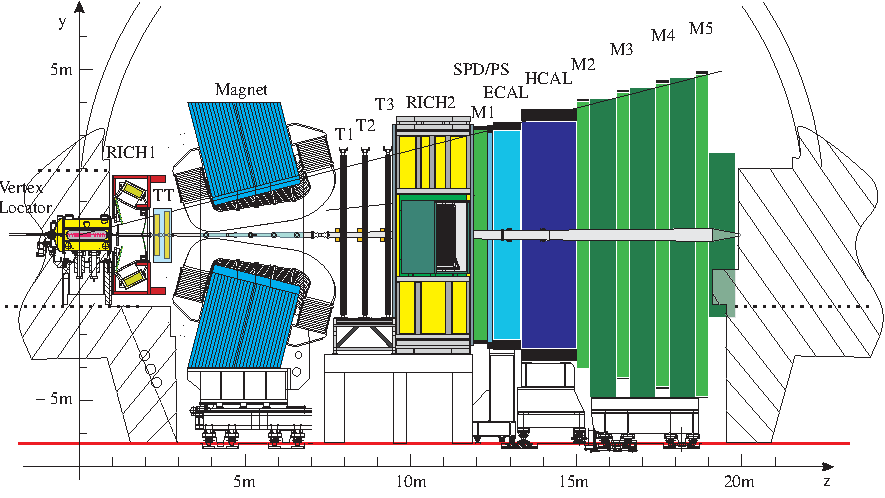
\includegraphics[width=\textwidth]{./figs-detector/lhcb_detector_view.pdf}
        \caption{The LHCb detector, run 1 and 2.}
    \end{subfigure}
    \hspace{12pt}
    %%%%
    \begin{subfigure}[t]{0.45\textwidth}
        \centering
        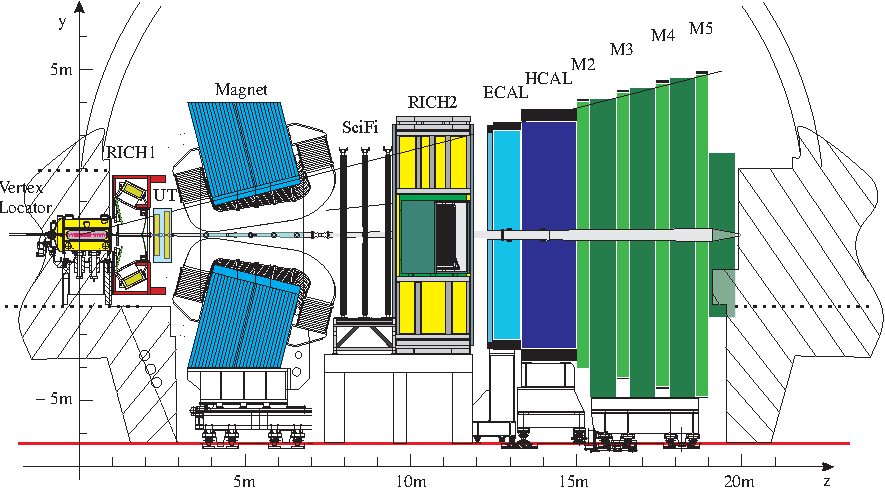
\includegraphics[width=\textwidth]{./figs-lhcb-upgrade-overview/lhcb_detector_view_run3.pdf}
        \caption{The upgraded LHCb detector in run 3.}
    \end{subfigure}

    \caption{
        The LHCb detector before (left) and after (right) LS2 upgrade.
        Note the upgrade on the tracking system:
        TT $\rightarrow$ UT, T-stations $\rightarrow$ SciFi;
        the removal of subdetectors relevant to L0 trigger only:
        the M1 muon station and SPD/PS have been removed.
    }
    \label{fig:lhcb-detector-comparison}
\end{figure}

The rest of the chapter provides an overview of the LHCb upgrade in LS2.
\Cref{ref:lhcb-upgrade-overview:trigger}
provides an comparison of the trigger schemes between run 2 and run 3.
The tracking and PID subdetectors are upgraded to provide better tracking
resolution and PID performance;
these will be discussed in \cref{ref:lhcb-upgrade-overview:tracking} and
\cref{ref:lhcb-upgrade-overview:pid}, respectively.


\section{Trigger schemes in run 2 and run 3}
\label{ref:lhcb-upgrade-overview:trigger}

As can be seen in \cref{fig:trigger-comp},
the main differences between run 2 and run 3 trigger scheme are:
the limited detector readout rate of 1~MHz is increased to 40~MHz\footnote{
    In the figure the frequency is labelled as ``30~MHz inelastic event rate''
    because it is the only type of collision that is visible to the LHCb
    detector.
    The readout rate is still 40~MHz, fully synchronous to the LHC frequency.
};
the storage write throughput is increased from 0.6~GB/s to 10~GB/s.
The implications of these differences are discussed in more details in the
following text.

\begin{figure}[!htb]
    \centering
    \begin{subfigure}[t]{0.36\textwidth}
        \centering
        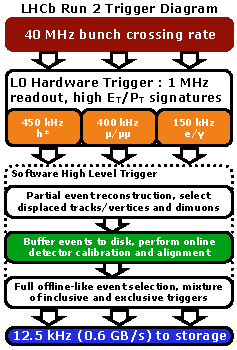
\includegraphics[width=\textwidth]{./figs-lhcb-upgrade-overview/trigger/trigger_scheme_run2.pdf}
        \caption{LHCb run 2 trigger scheme.}
    \end{subfigure}
    \hspace{20pt}
    %%%%
    \begin{subfigure}[t]{0.36\textwidth}
        \centering
        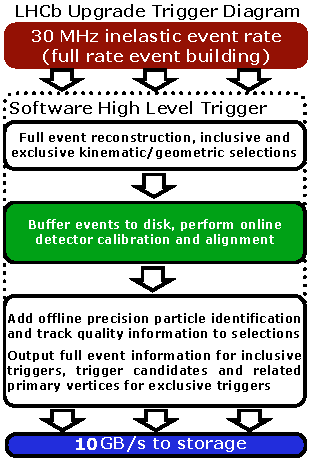
\includegraphics[width=\textwidth]{./figs-lhcb-upgrade-overview/trigger/trigger_scheme_run3.pdf}
        \caption{LHCb run 3 trigger scheme.}
    \end{subfigure}

    \caption{
        Comparison between run 2 and run 3 trigger schemes.
    }
    \label{fig:trigger-comp}
\end{figure}

The need for a higher readout rate at 40~MHz is due hadronic L0 trigger
saturation:
the hadronic L0 trigger requires the maximum energy $E_T$ deposited in the
calorimeters to be at least 3.7~GeV (for 2016) to reduce the triggering rate
at an acceptable level;
the threshold is already a significant portion of the $B$ meson mass
($\sim 5.3$~GeV).
Any further increase in luminosity requires an increase of the threshold,
which removes a significant portion of the signal events
that contain $B$ mesons,
resulting in an almost constant signal yield \cite{CERN-LHCC-2011-001}.

With a 40~MHz readout rate,
at 13~TeV with a pile-up of 5.2 (similar to run 3 condition),
the run 2 inclusive trigger strategy\footnote{
    To be clear, the run 2 trigger strategy contains both inclusive triggers,
    such as an inclusive $B$ trigger selecting a significantly displaced high
    \pt track forming a displaced vertex with 1--3 other tracks
    (referred as ``HLT2 topological trigger''),
    and exclusive triggers.
} of rejecting trivial backgrounds with
minimal bias cuts on few variables in an inclusive trigger is non-sustainable
for LHCb run 3:
assuming an event size of 100~kB\footnote{
    The original text uses kb (kilo-bit), which does not add up to 80~GB/s for
    a 800~kHz rate.
    The size should be in kB (kilo-byte), as supported in
    \cite{CERN-LHCC-2014-016,Allen_GPU_2020}.
    The 800~kHz number is reported in \cite{LHCb-PUB-2014-027}.
},
the write throughput for beauty hadrons is 27~GB/s, for charm it is 80~GB/s,
for light long-lived particles (such as $K^0_S$ and $\Lambda^0$) 26~GB/s
\cite{Albrecht_2014}.

However,
the write throughput is set to 10~GB/s,
due to limited LAN connection speed from the LHCb on-site online
system (responsible for data acquisition) to CERN's storage center (Tier0) in
Meryin\footnote{
    A small city near Geneva.
}, Switzerland.
According to \cite{CERN-LHCC-2014-016},
there are more than 20 pairs of fibers, each capable of transporting at 1~GB/s,
which, in theory, can provide a bandwidth of greater than 20~GB/s.
Still, in the same reference, a maximum write throughput of 10~GB/s is
considered, perhaps due to concerns on robustness.
%%%%
In any case, the 80~GB/s write throughput for a run 2-like inclusive trigger
strategy far exceeds the bandwidth capacity,
mainly due to the fact that with run 3 condition, a significant portion of
collisions contains genuine $B$ mesons.
Instead, it is preferable to employ a trigger strategy that categorize different
types of signals then apply cuts with as much information from an event as
possible, as early as possible
\cite{Albrecht_2014}.
Therefore, the full events are exposed directly to software HLT1 triggers which
reconstruct and select tracks with higher efficiency.

In general,
utilizing a software-only trigger allows more exclusive selections to reduce
bandwidth,
provides maximum flexibility,
and makes higher-level physics variables,
such as the invariant mass of a reconstructed vertex,
accessible to the trigger,
such that cuts can be applied directly on these variables,
reducing the need of cutting on proxy variables thus the need of modeling
acceptance effects offline \cite{Albrecht_2014}.

As a side note, the run 3 HLT1 trigger is entirely GPU-based\footnote{
    GPU: Graphics Processing Unit, as opposed to CPU: Central Processing Unit.
}, fully implemented
in CUDA \cite{Allen_GPU_2020},
as track reconstruction is ideally suited for parallel execution,
to which GPU is more advantageous than CPU:
while a CPU typically has highly frequencies, meaning it can execute more
``commands'' (instructions) in a given amount of time,
GPU, on the other hand, while having lower frequency, can execute the same
command on multiple input data\footnote{
    Modern CPU can also do this (Single Instruction, Multiple Data, SIMD),
    but the level of parallelism is not comparable to that of GPU:
    a modern CPU may allow simultaneous precessing of 8 data elements for a
    single SIMD core;
    for a 8-core CPU, it is capable of processing 64 data elements in parallel.
    Whereas a single GPU can handle as many as 5120 data elements
    (e.g. NVIDIA Tesla V100)!
    % https://www.cs.cmu.edu/afs/cs/academic/class/15418-s12/www/lectures/02_multicore.pdf
} in parallel.

In addition, the GPU-based solution is to save bandwidth:
There are about 250 event builders in the counting room to receive readout data
from the detector and assemble them into data packets suitable for software
triggers.
Had the HLT1 is purely implemented with conventional CPU programs,
the full detector readout (30--40~Tb/s, taken overhead into account) are
required to be sent out to the HLT farms.
Instead, a GPU-based HLT1 trigger exploits the fact that each event builder
can be equipped with 2 GPUs.
If the trigger can be implemented with less than 500 GPUs,
only events passing HLT1 cuts, which has a throughput of 1--2~Tb/s,
need to be sent out,
a factor of 30 reduction in bandwidth \cite{Allen_GPU_2020}.
The data transfer paths of a CPU- and GPU-based HLT1 are shown in
\cref{fig:cpu-vs-gpu-hlt1}.

\begin{figure}[!htb]
    \centering
    \begin{subfigure}[t]{0.36\textwidth}
        \centering
        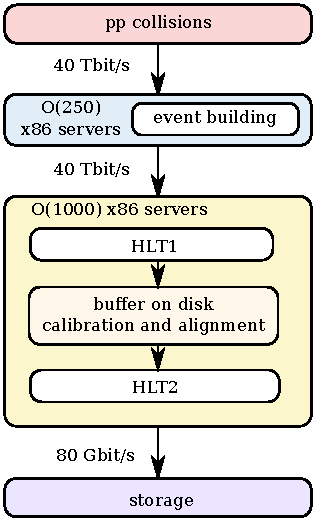
\includegraphics[width=\textwidth]{./figs-lhcb-upgrade-overview/trigger/data_path_cpu.pdf}
        \caption{CPU-based HLT1.}
    \end{subfigure}
    \hspace{20pt}
    %%%%
    \begin{subfigure}[t]{0.36\textwidth}
        \centering
        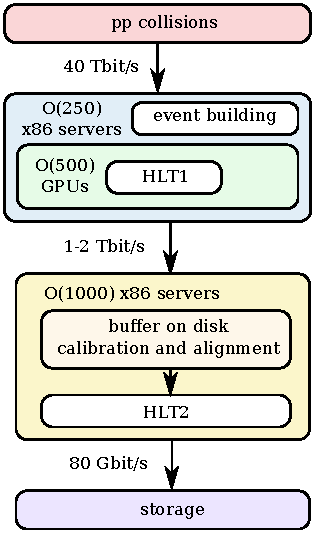
\includegraphics[width=\textwidth]{./figs-lhcb-upgrade-overview/trigger/data_path_gpu.pdf}
        \caption{GPU-based HLT1.}
    \end{subfigure}

    \caption{
        Comparison between data paths for a CPU- and GPU-based HLT1 trigger.
    }
    \label{fig:cpu-vs-gpu-hlt1}
\end{figure}

A recent benchmark, displayed in \cref{fig:allen-gpu-throughput},
shows that with about 200 high-end commercially available GPUs, the
30~MHz throughput of the LHCb readout can be sustained,
which is far below the 500 limit.
It also shows that the current HLT1 implementation scales linearly with
the performance of the GPU.
As more performant GPU emerges, more powerful HLT1 algorithms may be implemented
with less number of GPUs.

\begin{figure}[!htb]
    \centering
    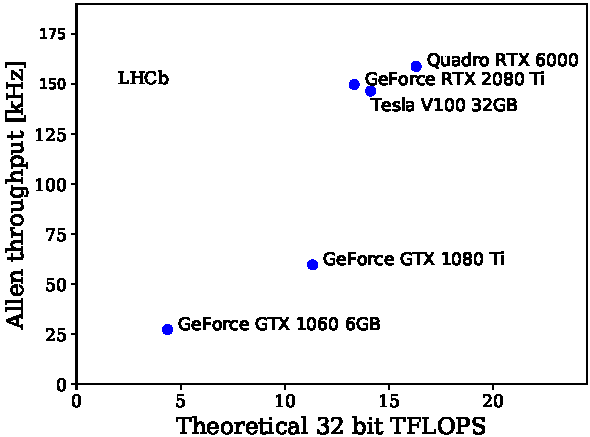
\includegraphics[width=0.5\textwidth]{./figs-lhcb-upgrade-overview/trigger/allen_perf_vs_tflop.pdf}
    \caption{
        GPU-based HLT1 throughputs on many GPUs with respect to their reported
        peak 32-bit TFLOPS (Tera Float Point Operation Per Second) performance.
        Taken from \cite{LHCB-FIGURE-2020-014}.
    }
    \label{fig:allen-gpu-throughput}
\end{figure}


\section{Tracking system}
\label{ref:lhcb-upgrade-overview:tracking}

All subdetectors of the tracking system undergo significant upgrade to improve
resolution and radiation hardness, aside from the required upgrade to their
readout system.

\begin{figure}[!htb]
    \centering
    \begin{subfigure}[t]{0.72\textwidth}
        \centering
        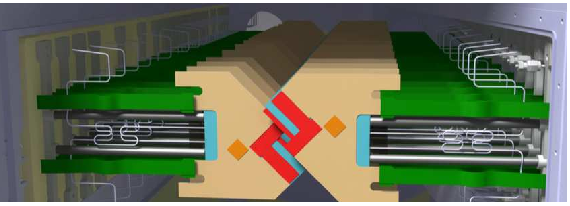
\includegraphics[width=\textwidth]{./figs-lhcb-upgrade-overview/tracking/velo_upgrade.pdf}
        \caption{Upgraded VELO.}
        \label{fig:velo-upgrade}
    \end{subfigure}

    %%%%
    \begin{subfigure}[t]{0.48\textwidth}
        \centering
        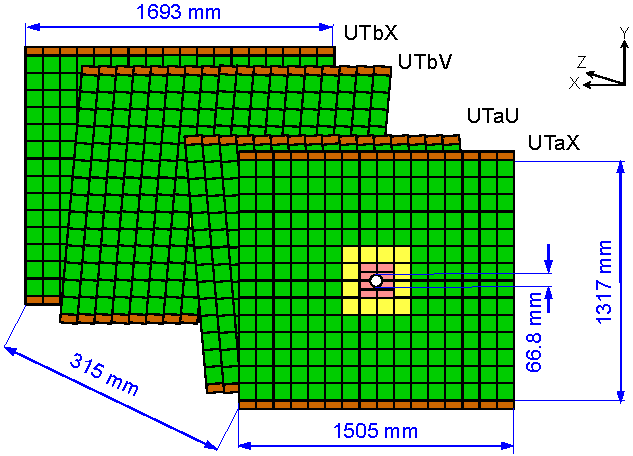
\includegraphics[width=\textwidth]{./figs-lhcb-upgrade-overview/tracking/ut_upgrade.pdf}
        \caption{The UT, which replaces TT.}
        \label{fig:ut-upgrade}
    \end{subfigure}
    \hfill
    \begin{subfigure}[t]{0.48\textwidth}
        \centering
        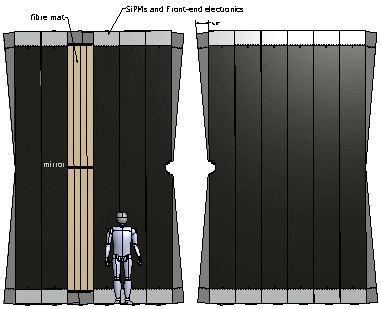
\includegraphics[width=\textwidth]{./figs-lhcb-upgrade-overview/tracking/scifi_upgrade.pdf}
        \caption{The SciFi tracker, which replaces T-stations.}
        \label{fig:scifi-upgrade}
    \end{subfigure}

    \caption{
        Upgraded tracking system of the LHCb detector.
    }
\end{figure}

The upgraded VELO detector is now a 26-layer pixel\footnote{
    As opposed to silicon strip, which consists of thin long metal strips
    implant on silicon wafer,
    pixel are typically of finer square shape.
} tracker with a pixel size of $50 \times 50$~$\upmu$m$^2$,
placed even closer to the beam at 5.1~mm,
and has less detector materials, from 4.6\% to 1.7\% radiation lengths, before
particles hit the first tracking layers which is crucial to improve the
resolution on the impact parameters (IP) \cite{Hennessy_2017}.
A single layer of the upgraded VELO detector is shown in
\cref{fig:velo-upgrade}.
The improvement in IP resolution based on simulation is shown in
\cref{fig:velo-ip-improvement}.

\begin{figure}[!htb]
    \centering
    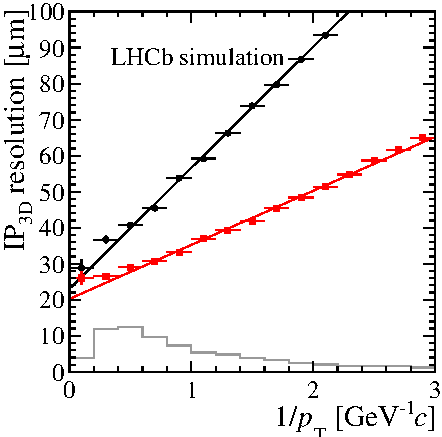
\includegraphics[width=0.4\textwidth]{./figs-lhcb-upgrade-overview/tracking/velo_ip_improvement.pdf}
    \caption{
        The upgraded VELO provides better IP resolution, based on simulation.
        The IP resolution for current (\textbf{black}) and upgraded
        (\textcolor{red}{\textbf{red}})
        VELO are both evaluated at a
        pile-up of 7.6 and a center of mass energy of 14~TeV, a typical run 3
        condition.
    }
    \label{fig:velo-ip-improvement}
\end{figure}

The Tracker Turicensis (TT) is replaced by the Upstream Tracker (UT).
Located immediately before the Magnet,
UT will be used for reconstructing long-lived particles decaying after VELO.
It improves the momentum resolution of long tracks and trigger timing,
as well as reducing fake tracks
\cite{Piucci_2017,Wang:2015mem}.
Still based on silicon-strip technology, UT has a smaller pitch near the beam
pipe:
180~$\upmu$m in the peripheral and 95~$\upmu$m around the beam pipe,
and sits closer to the beam.
UT has identical geometry to that of TT:
4 planes of sensors arranged in a $x$-$u$-$v$-$x$ configuration,
as shown in \cref{fig:ut-upgrade}.
Compared to TT, UT provides sufficient radiation hardness,
reduces occupancy in the critical region near the beam, and improves
\pt resolution \cite{LHCB-TDR-015},
as displayed in \cref{fig:ut-pt-improvement}.
More details regarding UT will be provided in \cref{ref:ut}.

\begin{figure}[!htb]
    \centering
    \begin{subfigure}[t]{0.48\textwidth}
        \centering
        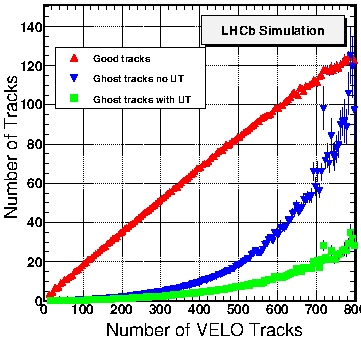
\includegraphics[width=0.82\textwidth]{./figs-lhcb-upgrade-overview/tracking/ut_ghost_improvement.pdf}
        \caption{
             Requiring hits on at least 3 out of 4 UT planes for tracks within
             the UT fiducial volume reduces fake tracks significantly.
        }
    \end{subfigure}
    \hspace{10pt}
    \begin{subfigure}[t]{0.48\textwidth}
        \centering
        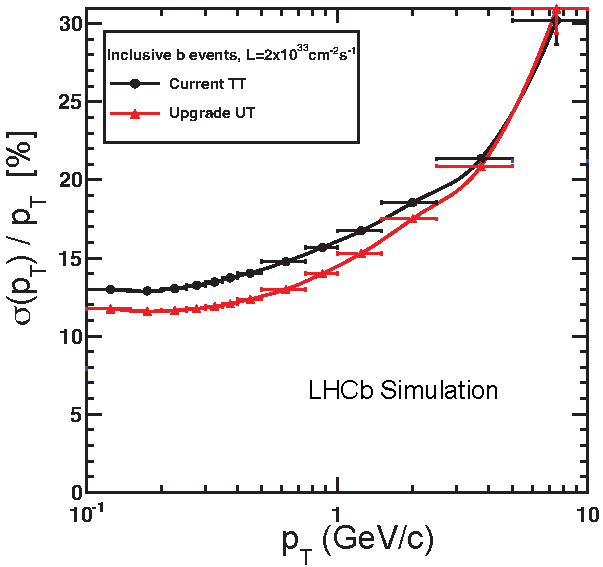
\includegraphics[width=0.82\textwidth]{./figs-lhcb-upgrade-overview/tracking/ut_pt_improvement.pdf}
        \caption{
            Compared to TT,
            UT provides better \pt resolution, especially at lower \pt.
        }
    \end{subfigure}
    \caption{
        UT provides better \pt resolution to the long tracks and reduces fake
        (ghost) tracks.
        Figures taken from \cite{Wang:2015mem}.
    }
    \label{fig:ut-pt-improvement}
\end{figure}

The Scintillating Fiber tracker (SciFi), replacing T-stations,
constructed from $3 \times 4$ detector layers,
are placed after the Magnet to provide track and momentum
reconstruction for the downstream tracks.
Each layer of SciFi is composed of 6 layers of 2 set of
2.4~m long plastic scintillating fibers with 250~$\upmu$m diameter arranged
vertically, separated by a mirror in the middle.
One layer of SciFi is 1.35~mm thick and has a surface area of $6 \times
5$~m$^2$.
The fibers are readout with Silicon PhotoMultipliers (SiPM), located at the top
and bottom of the detector,
with a pixel size of $57 \times 62$~$\upmu$m$^2$
\cite{Piucci_2017,Massafferri_2020}.
The spatial resolution of the SciFi is better than 100~$\upmu$m
\cite{Massafferri_2020}.
A diagram illustrating the general operating principle of SciFi is displayed
in \cref{fig:scifi-op}.

\begin{figure}[!htb]
    \centering
    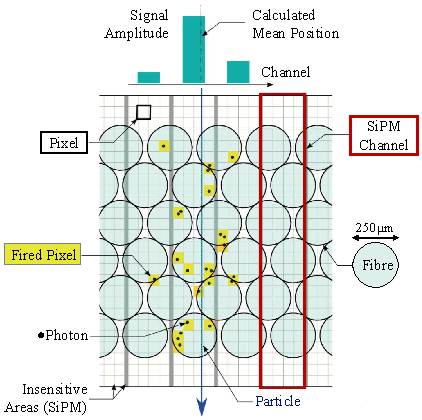
\includegraphics[width=0.5\textwidth]{./figs-lhcb-upgrade-overview/tracking/scifi_op_principle.pdf}
    \caption{
        Operation principle of SciFi.
        Taken from \cite{Berninghoff:2810671}.
    }
    \label{fig:scifi-op}
\end{figure}


\section{Particle identification system}
\label{ref:lhcb-upgrade-overview:pid}

In run 2 the occupancy for RICH1 can reach 30\%,
the upper limit of good PID performance.
A factor of 5 increase in luminosity in run 3 would certainly degrade the PID
performance.
To mitigate the problem,
the photon distribution is spread over a wider area by increasing the
radius of the spherical mirrors to 3.7~m (as opposed to 2.7~m in run 2).
In addition, the focal plane is moved back which leads to an enlargement
of the Cherenkov ring size
\cite{D_Ambrosio_2017,Okamura:2837863}.

The photon detection system for both RICH detectors are upgraded from
Hybrid Photon Detectors (HPDs) to Multi-anode PhotoMultiplier Tubes (MaPMTs)
to provide single-photon counting ability at 40~MHz
\cite{Okamura:2837863}.
